\documentclass[letterpaper, DIV=11]{scrartcl}

\usepackage{polyglossia}
\setdefaultlanguage{french}

\usepackage[backend=biber]{biblatex}
\addbibresource{../../elecmag.bib}

\usepackage{fontspec}
\setmainfont[Renderer=Basic, Numbers=OldStyle, Scale = 1.0]{TeX Gyre Pagella}
\setsansfont[Renderer=Basic, Scale=0.90]{TeX Gyre Heros}
\setmonofont[Renderer=Basic]{TeX Gyre Cursor}

\setkomafont{title}{
  \normalfont
  \itshape
  \rmfamily
}
\addtokomafont{author}{
  \itshape
}
\addtokomafont{date}{
  \itshape
}
\setkomafont{section}{
  \normalfont
  \itshape
  \rmfamily
  \Large
}

\usepackage{booktabs}
\usepackage{graphicx}
\usepackage{enumitem}
\usepackage{tikz}
\usepackage{amsmath}
\usepackage[locale=FR]{siunitx}
\usepackage{hyperref}

\sisetup{
  mode=text,
  reset-text-family=false,
  reset-text-series=false,
  per-mode=symbol,
  uncertainty-mode=separate,
}

\newcommand{\F}{\boldsymbol{\vec{F}}}
\newcommand{\vv}{\boldsymbol{\vec{v}}}
\newcommand{\va}{\boldsymbol{\vec{a}}}


\title{Prélaboratoire -- Loi d'Ohm}
\author{}
\date{}

\begin{document}

\maketitle

Pour préparer le laboratoire sur la loi d'Ohm, lisez attentivement les documents suivants
\begin{itemize}
  \item section \textit{Instruments de mesure} du Guide de laboratoire;
  \item protocole \textit{Labo 1 -- Loi d'Ohm} du Guide de laboratoire;
  \item protocole \textit{Utilisation de la source GW Instek GPS} disponible sur Léa.
\end{itemize}

Répondez ensuite aux questions ci-dessous dans votre cahier de laboratoire.
Pour les schémas à compléter, vous pouvez imprimer les images ci-dessous et les
coller dans votre cahier de laboratoire ou les reproduire à la main.


\begin{enumerate}
  \item Quel appareil servira de source de tension?
  \item Quel appareil utiliserez-vous comme ohmmètre?
  \item Quel appareil utiliserez-vous comme ampèremètre?
  \item Quel appareil utiliserez-vous comme voltmètre?
  \item Considérez la mesure de la résistance de la céramique. Faites un schéma
    technique du circuit, puis complétez la figure ci-dessous en dessinant les
    connexions que vous devrez faire.

    \begin{center}
    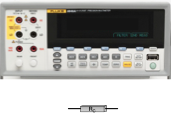
\includegraphics{figures/fluke_resistance_ceramique.png}
    \end{center}

  \item Considérez le circuit complet incluant la céramique, l'ampoule et la
    source de tension. Vous voulez prendre les mesures de courant et de
    différence de potentiel aux bornes de l'ampoule. Faites un schéma technique
    du circuit, puis complétez la figure ci-dessous en dessinant les connexions
    que vous devrez faire.

    \begin{center}
    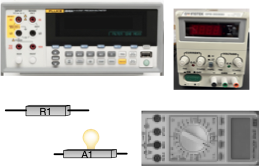
\includegraphics{figures/circuit_complet.png}
    \end{center}

  \item Vous avez mesuré un courant de \qty{52.3451}{\milli\ampere} avec le
    multimètre identifié à la question 3. Sachant que l'échelle du multimètre
    lors de la prise de mesure était celle de \qty{100}{mA}, quelle est
    l'incertitude sur la mesure? Écrivez le résultat du mesurage en respectant
    toutes les règles d'écriture.
\end{enumerate}


\printbibliography


\end{document}


